\chapter{Teorie}
\label{2-Teorie}

\section{OpenStreetMap}
\label{OpenStreetMap}

\subsection{Vznik}
\label{vznik}
OpenStreetMap (OSM) je projekt, jež vznikl s cílem vytvoření a sběru 
volně dostupných geografických dat a následně jejich možné vizualizace
do topografických map. Projekt založil Steve Coast v červenci roku 
2004 v Anglii. Jako inspirace mu posloužil projekt Wikipedia.

Zprvu projekt využívalo jen pár nadšenců, postupem času ale získal
projekt popularitu. S nárůstem počtu uživatelů se zvyšoval i objem dat.
Bylo tedy nutné navýšit kapacitu a zabezpečení serverů.
Také bylo potřeba zlepšit síťové řešení a infrastrukturu.
Tím je myšleno, že data byla rozdělena na více serverů, aby se rozložila zátěž na ně.
 
%%% ML: nejen kapacitu serveru, ale cele infrastruktury, resit dalsi otazky (bezpecnost a pod)...

V dubnu roku 2006 byla založena nadace OpenStreetMap Foundantion pro financováni 
projektu jako takového (zaměstnanců, běhu a zajištění bezpečnosti serverů atd.). \cite{wikiOSM}


\subsection{Struktura dat}
\label{struktura dat}
OSM data jsou nyní uložena v databázi PostgreSQL. \footnote{viz \url{http://blog.cleverelephant.ca/2009/04/openstreetmap-moves-to-postgresql.html}}

%%% primo v DB, cemuz tak ale neni; XML, resp. OSM je vymenny format
Pro samotnou výměnu dat ale slouží souborový formát {.osm}, který využívá datový
formát  XML. 
Jeho výhoda je jasná struktura, snadná orientace v kódu pro člověka. 
Nevýhodou je ovšem větší objem dat, který lze ale snížit kompresí. 

%%% ML: tady by se hodil vycet (itemize), chtelo by do vysvetlit, co je cesta a pod...
Elementy jsou v OSM rozděleny na: uzel (node), cesta (way) a
relace (relation).

Příklad XML souboru pro cestu:

{\scriptsize
\begin{lstlisting}
<osm version="0.6" 
generator="CGImap 0.4.0 (32632 thorn-01.openstreetmap.org)" 
copyright="OpenStreetMap and contributors" 
attribution="http://www.openstreetmap.org/copyright" license="http://opendatacommons.org/licenses/odbl/1-0/">

   <way id="87249754" visible="true" version="2" changeset="34489106"
        timestamp="2015-10-07T11:52:41Z" user="Petr Dlouhý" uid="17615">
       <nd ref="1014526199"/>
       <nd ref="1014525941"/>
       <nd ref="1014526337"/>
       <nd ref="1014526022"/>
       <nd ref="1014526277"/>
       <nd ref="1014525984"/>
       <tag k="highway" v="path"/>
       <tag k="source" v="bing:ortofoto"/>
   </way>
</osm>
\end{lstlisting}
}


Základním bodovým elementem je uzel (node), který je definován jedinečným
identifikátorem ({\tt id=}). Všechny souřadnice jsou ve WGS~84 (EPGS 4326). 
Je také ukládána verze ({\tt version= }), to jest, kdy byl do databáze přidán
a také zde je uvedeno v jaké změně to bylo provedeno ({\tt changeset=~}).
%%% ML: opet cestina (minimalne 2x "a")... preformulovat
Dále je možné připojit různé atributy s klíčem a hodnotou ({\tt tag~k=~v=~}).
Příklad atributu pro strom: {\tt tag k='natural' v='tree'}.
%%% ML: cely tento odstavec plati i pro dalsi elementy - way/area (?)

Další liniový element je cesta (way) a ta je vždy spojení dvou a více uzlů.
Ta má také svůj jedinečný identifikátor ({\tt way~id=~}) v rámci všech cest.
Má vždy základní atributy jako {\tt id=*, visible=*, version=*, .. }, 
stejně jako u elementu uzel.
Dále však musí být seznam bodů, ze kterých se skládá.
Je zde uvedena pouze reference na id bodů, nikoliv jejich souřadnice.
Cestám lze taktéž přiřadit různé atributy.

Cesty se dále rozdělují na neuzavřené a uzavřené. Uzavřeným cestám se dají přidat
i atributy určené jen pro plochy. Například les ({\tt landuse=forest}).

Speciálním elementem je relace (relation), do které lze zahrnout
jeden a více elementů. Mohou se do nich spojit elementy stejného (uzel a uzel),
nebo různého druhu (uzely, cesty nebo i relace). 
Například dálnice je tvořena několika cestami (way), a ty
jsou zahrnuty do společné relace Dálnice D1. Nebo například turistická trasa
(od~KČT) může být relace sdružující jak liniové elementy (cesty, pěšiny) tak i bodové
(rozcestníky, vyhlídky, apod. ).

%%% ML: osm wiki zni familiarne, + reference v tomto pripade je lepsi
%%% hned za slovem, nemusim byt na konco odstravce
U atributů popsaných na OpenStreetMap Wikipedii \cite{OSMfeatures} je vždy uvedeno, k jaké třídě je
vhodné a nevhodné je použít (dle komunity uživatelů OSM). Pokud se stane, že je použit
na~jinou než povolenou třídu, může být následně problém v některých vykreslovačích. 
%%% ML: viz kapitola?

\subsection{Změna licence}
\label{změna licence}

Původně byla data OSM a generované grafické dlaždice distribuována pod licencí
Creative~Commons~AllributionShare~Alike 2.0 (CC~BY~SA~2.0).

Tato licence umožňovala užití (distribuci ale i editaci) díla pod podmínkou,
že bude uveden zdroj OpenStreetMap.org ve viditelné části
vytvořených mapových dlaždic \cite{OSMlicence}.

  \begin{figure}[hbt]
    \centering
      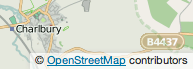
\includegraphics{./pictures/attribution_example.png}
      \caption{Příklad umístění licence}
      \label{fig:attribution_example}
  \end{figure} 
%%% ====================================
%%% ML: duvod zmeny ?
V roce 2012 byla licence publikovaných dat změněna na Open Data Commons
Open Database Licence (ODbL).
Tato změna licence přinesla problém
s~daty, které byly poskytnuty projektu v předchozí licencí
(CC~BY~SA~2.0). Bylo nutné se dotázat každého z dřívějších
přispěvatelů dat, ať už právnických osob, tak i fyzických osob, jestli
%%% ML: slo o to, zda souhlasi aby jejich prispevky byly poskytovany
%%% pod novou licenci, veta to naznacuje, ale je nepresna
s touto změnou souhlasí a je možné s jejich daty i s novou licencí
nakládat. U přispěvatelů, kteří nedovolili užívání jejich díla
%%% ML: co vymazat - jejich prispevky - preformulovat
pod novou licencí, nebo u těch, co se nevyjádřili, bylo nutné
%%% ML: chybi reference, co znamena zlomek?
z~databáze vymazat. Tato situace nastala pouze ve zlomku případů.
%%% ML: v jake mire? doplnit
Nejvíce tato změna licencí ohrozila data v zemích jako je Polsko a Nový Zéland.

%%% ML: proc tento dualismus?
V současnosti jsou tedy data OSM distibuována pod licencí ODbL a
generované grafické dlaždice pod licencí CC-BY SA 4.0
\cite {OSMlicenceIssue}.

\subsection{Licence ODbL}

%%% ML: preformulovat: Licence ODbl umoznuje...
Ve zkratce s daty pod licencí ODbL uživatel smí:
\begin{itemize}
    \item    kopírovat, distribuovat a užívat data
    \item    vytvářet nová data z původních
    \item    měnit původní data
\end{itemize}

%%% ML: preformulovat
S použitím ale uživatel musí ale uvést zdroj a licenci dat.
Dále uživatel souhlasí, že nová data vytvořená z původních dat budou sířena
také pod~licencí ODbL.
Podrobněji viz přesné znění licence na stránkách OpenDatabase.\footnote{\url{http://opendatacommons.org/licenses/odbl/1.0/}}


\subsection{Zdroje dat}
\label{Zdroje dat}
Jak bylo zmíněno, byla snaha, aby mapová data tvořili jedinci prvotním
sběrem dat, tj. měřením vlastními GNSS (GPS, Glonass) přijímači a
znalostí místních poměrů (uzavřené silnice, stezky atd.).  A takto
vzniklé dílo volně užívat k vlastním potřebám.  Komunita přispěvatelů se
zprvu pomalu, později poměrně rychle rozrostla a dnes čítá 3,7 milionů
registrovaných uživatelů s alespoň jednou vytvořenou změnou v OSM a
2,7 milionů účtů aktivních přispěvatelů.\cite{OSMstats}

Takto vzniklé mapové podklady byly velice vhodné i pro další projekt, dnes již
velice rozšířený a známý jako Geocashing (GC). Projekt GC začal mapové
podklady od OSM užívat a zároveň jeho uživatelé začali sami tvořit a
přispívat do OSM. 

Přispěvatelé dat do OSM musí respektovat licenci projektu OdbL.
Tudíž i jejich zdroj dat musí splňovat tuto licenci. Proto by měli
všechny svoje změny, které v OSM vytvoří, řádně ozdrojovat atributem
s~klíčem 
{\tt source}.
V případě vlastního sběru dat se vyplňuje hodnotou
{\tt source=survey} ,
popřípadně uvést zdroj, odkud čerpali. Pokud tuto povinnost poruší a
použijí zdroj, jež není kompatibilní s licenční politikou OSM, tak ostatní přispěvatelé do OSM tuto změnu, aby předešeli sporům, odstraní. V tomto případě dojde k odstranění celé sady změn, byť by v~ní byl pouze jeden prvek, jenž toto poruší.

%%% ML: nejen soukrome, ale i statni organizace, viz CUZK s RUIANem,
%%% OK mate to v dalsi odstavci
Druhým významným zdrojem dat jsou soukromé subjekty (společnosti).
Většinou jde o podkladové zdroje dat, například ortofoto. Pro obkreslování
silničních síti z~leteckých nebo satelitních snímků. V~jejich případě to
bylo řešeno písemným svolením, nebo smlouvou. Jako významným zdrojem byla
%%% ML: a ted uz neni...? Bing je spolecnost, nevlastni ji MS?
společnost Bing, jež nabídla k~dispozici letecké snímky většiny
obydlené pevniny. 

Třetím zdrojem dat a zároveň postupně dominujícím, co do jeho obsahu, jsou
%%% ML: ze -> produkované
datové sady ze státního sektoru. Tyto datové sady jsou nejvhodnějším zdrojem
%%% ML: proc ? vyargumentovat
dat.

\subsection{Importy}
\label{Importy}
Výraz import v tomto případě znamená začlenění většího množství datových sad
z~jednoho datového úložiště (databáze serveru) na jiný. Při velkých objemech dat
se využívá výkonu výpočetní techniky z důvodu její bezchybovosti, a také
z~důvodu časové náročnosti. Na člověku poté ale zbývá zvolit postup importu
a naprogramovat skript nebo program, podle něhož technika samotný proces
provede. 

Datové importy z veřejných databází do databáze OSM jsou velmi cenné. 
Otevřené geografické, ale i jiné, databáze státu a jeho veřejných institucí 
financovaných státem jsou komplexní. Komplexní v tom smyslu, že obsahují celistvý
soubor dat, protože je daná instituce vyžaduje ke svém chodu. Jistá nevýhoda tu 
ale může být, a to, že data nemusí být vždy úplně aktuální. Některá data mohou 
být sbírána a zveřejněna i s větším časovým odstupem.

V rámci České Republiky proběhlo již několik hromadných datových importů. Jak 
již bylo řečeno, větší časová náročnost zabere samotná příprava na import. A to
v~případě, importu do OSM. Nejen napsání skriptu, ale i nutná diskuze tohoto záměru
na~diskuzní konferenci Talk-cz. 

\subsection{Talk-cz}
\label{Talk-cz}
Tato diskuze probíhá přes posílání emailových zpráv do společné konference. 
Uživatelům chodí emaily z probíhající diskuze a pokud na nějaký chtějí reagovat,
tak pošlou email na adresu serveru, na kterém diskuze běží, a musí do Předmětu 
napsat Re: a předmět zprávy, na kterou reagují. Server tyto zprávy pomocí 
předmětu a času řadí. Diskuze je poté k dispozici na webových stránkách.\footnote{http://lists.openstreetmap.org/listinfo/talk-cz}

\subsection{Vykreslovače}
\label{Vykreslovače}
Na hlavní stránce OSM (\url{http://www.openstreetmap.org}) je k dispozici mapová aplikace. Ta nabízí pět
„základních“ přednastavených vrstev vykreslených z~dat z OSM. Mapová
%%% ML: na cem je zalozen AJAX, kdyz uz to zminujete. Vysvetlit anebo odstranit.
aplikace OSM využívá knihovnu OpenLayers založenou na konceptu AJAX.
%%% ML: jde o EPSG:3857 - zminit, stejny souradnicovy system pouziva
%%% Google Maps a pod.
Pro snadné vykreslení dat do grafických dlaždic se používá Mercatorovo
zobrazení.

%%% ML: mozna dodat screenshoty do prilohy?
\begin{itemize}

  \item Standardní vrstva - vykresluje všechny prvky přiměřeně.
  \item Cyklomapa - vykresluje cyklostezky, výškopis. 
  \item Dopravní mapa - vykresluje silniční a železniční sítě.
  \item MapQuest Open - podkladová mapa právě pro potřeby 
    Geocaching.
    %%% ML: restaurace na prvni miste?
  \item Humanitární mapa, která vykresluje služby (restaurace, banky, muzea, 
  školy, kostely...)  a potlačuje ostatní prvky. 

\end{itemize}

%%% ML: kompozici? ruznych dat? dovysvetlit
Existují další stránky, jež se zabývají vlastní kompozicí a vykreslením
různých dat. Například mapu turistických a cyklistických tras vykresluje
pro celou Evropu mtbmap.\footnote{mtbmap.cz}

%%% priklad? mozna dodat hezky screenshot?
Zajímavými projekty jsou například ty, které k 2D mapě přidávájí „třetí“ rozměr a
vytvářejí tzv. 2.5D mapu. Většinou jde o 3D zobrazení budov, mostů (dle
atributů), popřípadě i stromů.

\section{Opendata}
\label{opendata}

%%% ML: od kud toto cerpate. Otevrena data (ala public domain) maji
%%% svuj puvod mnohem drive, v devadesatych letech...
Základní myšlenka otevřených dat vznikla v USA z iniciativy vlády Barracka Obamy.
%%% ML: nejen geograficka data
Tedy pokud vzniknou geografická data z veřejných peněz, měla by tedy být
%%% ML: tady neco tvrdite, ale nemate to podlozeno
přístupná veřejně. Mělo to kladný efekt na tamní ekonomiku. Díky tomuto byly
%%% ML: Landsat a SRTM jsou zverejnena jiz delsi dobu... to opravdu
%%% nesouvisi s vladou BO
zprvu k~dispozici satelitní snímky povrchu Země a digitální model terénu
s~rozlišením 30x30 m od NASA (pro pozdější vykreslení vrstevnic).

Tento trend se začal rozšiřovat zprvu do zemí západní Evropy,
%%% ML: druha cast vety nenavazuje na prvni, jake zeme, opet, nejaka
%%% reference?
jmenovitě Velké Británie, Francie či Německa, ale i jiné země mimo Evropu..

%%% ML: Fond se jmenuje Fond Otakara Motejla (opravdu jej zalozil on,
%%% nebyl zalozen na jeho pocet). Jednim z projektu fondu jsou prave
%%% Otevrena data
V ČR se tomuto věnuje fond Otevřená data\footnote{www.otevrenadata.cz}, který založil Otakar
%%% ML: Sociery? co Rekostrukce statu a pod.?
Motejl. Tento fond spolupracuje s nadací Sociery Fund Praha. V rámci
těchto uskupení je vyvíjen tlak na transparentnost veřejné správy a
zveřejňování smluv a dat
státních institucí, jelikož jejich získání a údržba byla placena
z~veřejných zdrojů.

\section{IPR Praha}
\label{IPR Praha}
IPR Praha je zkratka názvu Institut plánování a rozvoje a hlavního města Prahy. 
Tento institut se věnuje urbanismu, architektury a rozvoje města Prahy. Hlavním
úkolem IPR je tvorba územního plánu Prahy a významným úkolem IPR je zajišťovat
zpracování geografických informací. Spravuje data a mapy města Prahy. Od roku 
2002 poskytuje na svých stránkách zdarma webové aplikace bez limitu využití. 
Po~rozvoji Pražského geoportálu došlo k jejich většímu využívání.  Na základě 
platných Pravidel pro poskytování dat a  výstupů z datových souborů a datového 
skladu Geografického byla od dne 1.~4.~2015 zveřejněny datové soubory a další 
webové služby. Tato data byla uveřejněna pod licencí CC-BY SA 4.0 \cite{IPR}
\subsection{licence CC BY-SA 4.0}
\label{licence CC BY-SA 4.0}
Licence CC BY-SA 4.0 je zde uvedena ve zjednodušeném znění.

"Uživatel s smí
\begin{itemize}
    \item   Sdílet - rozmnožovat a distribuovat materiál prostřednictvím jakéhokoli média v jakémkoli formátu
    \item   Upravovat - remixovat, změnit a vyjít z původního díla
\end{itemize}
pro jakýkoliv účel, a to i komerční.

Poskytovatel licence nemůže odvolat tato oprávnění do té doby, dokud dodržujete licenční podmínky.

Uveďte původ — Je Vaší povinností uvést autorství, poskytnout s dílem odkaz na licenci a vyznačit Vámi provedené změny. Toho můžete docílit jakýmkoli rozumným způsobem, nicméně nikdy ne způsobem naznačujícím, že by poskytovatel licence schvaloval nebo podporoval Vás nebo Váš způsob užití díla.

Zachovejte licenci — Pokud budete toto dílo upravovat, pozměňovat nebo na něj navazovat, musíte svoje odvozená díla vystavovat pod stejnou licencí jako původní dílo."

Podrobněji viz přesné znění na stránkách CraetiveCommmons.
\footnote{https://creativecommons.org/licenses/by-sa/4.0/legalcode/}
